\section{Представление геометрической информации в различных видах ПО}\label{sec:geoDifferentReprs}

% ================================================================================================================
%   ____    _    ____                                      _              
%  / ___|  / \  |  _ \      __ _  ___  ___  _ __ ___   ___| |_ _ __ _   _ 
% | |     / _ \ | | | |    / _` |/ _ \/ _ \| '_ ` _ \ / _ \ __| '__| | | |
% | |___ / ___ \| |_| |   | (_| |  __/ (_) | | | | | |  __/ |_| |  | |_| |
%  \____/_/   \_\____/     \__, |\___|\___/|_| |_| |_|\___|\__|_|   \__, |
%                          |___/                                    |___/ 
% ================================================================================================================

\subsection{Граничное представление BREP}\label{sec:geoCAD}

Граничное представление (Boundary representation, BREP) --- наиболее распространённый способ точного описания геометрии в ЭВМ, используемый геометрическими ядрами всех современных систем автоматизированного проектирования (САПР).
% Похоже, это первое явление САПР и CATIA народу в тексте (не во всяких списках типа цели, новизна и проч.)
Во многих физических лабораториях, включая CERN, GSI и ОИЯИ, в качестве основной САПР используется система CATIA~v5 (Computer-Aided Three-dimensional Interactive Application), разрабатываемая французской фирмой Dassault Systemes.

\textbf{Далее представление геометрической информации в САПР мы будем называть просто BREP, хотя строго говоря это не совсем верно.}

% Ссылка на Голованова должна появиться где-то
% \todo
Геометрическое моделирование в САПР и граничное представление достаточно подробно описаны в работе~\cite{Golovanov}.

В BREP есть два типа понятий --- геометрические (<<точка>>, <<кривая>>, <<поверхность>>) и топологические (<<вершина>>, <<ребро>>, <<грань>>). <<Точка>> --- это тройка координат в некоторой системе координат. <<Кривая>> --- это уравнение, задающее множество точек, принадлежащих данной кривой. Кривую удобно описать с помощью параметрического уравнения от одной переменной. <<Поверхность>> --- это уравнение, задающее множество точек, принадлежащих данной поверхности. Соответственно, поверхность удобно описать с помощью параметрического уравнения от двух переменных. Топологические сущности задаются на базе геометрических. <<Вершина>> лежит в некоторой геометрической точке. <<Ребро>> лежит на некоторой геометрической кривой и ограничено двумя вершинами. Очевидно, что эти вершины должны принадлежать кривой, то есть и соответствующие геометрические точки должны принадлежать кривой. <<Грань>> лежит на некоторой поверхности и ограничена замкнутым циклом из рёбер. Также очевидно, что эти рёбра должны принадлежать поверхности, как и кривые, на которых они лежат, как и вершины и точки, ограничивающие эти рёбра. Замкнутая оболочка из граней с указанием внешних сторон этих граней ограничивает некоторую область пространства, называемую <<телом>>.

В памяти ЭВМ или обменном файле создаётся древовидная структура. Терминальными вершинами этого дерева чаще всего являются геометрические точки, представляющие собой тройки чисел с плавающей точкой. Далее вверх по дереву, имеются узлы типа вершина со ссылками на геометрические точки. Ребро также представляется в виде узла дерева, от которого идёт ссылка на геометрическую сущность, описывающую уравнение кривой, на которой это ребро построено, и ссылки на вершины, ограничивающие это ребро.

В соответствии с BREP параллелепипед (которому эквивалентен примитив box в CSG, см. секцию~\ref{sec:secGeoCSG}) задаётся следующим образом (\figref{fig:BREPbox1} и \figref{fig:BREPbox2}). На этих рисунках дерево представленно упрощённо. Имеется 8 вершин, каждое из 12 рёбер ограничено двумя из этих восьми вершин. Описание вершин не дублируется, на одну и у же сущность может быть множество ссылок. Аналогичным образом каждая из 6 граней ограничена прямоугольником --- циклом из четырёх рёбер, поэтому от каждой сущности типа грань идёт 4 ссылки на рёбра. Тело представляется как замнутая оболочка из поверхностей, поэтому от сущности типа solid идут ссылки на 6 граней. Фактически, помимо представленной на рисунках структуры, имеется ещё довольно-таки много дополнительной информации, без которой корректное и однозначение описание было бы невозможным, например, направления рёбер, направления обхода в цикле из рёбер, направления нормалей граней, уравнения кривых и поверхностей (в данном примере лишь неявно, т.к. используются базовые прямые линии и плоскости), и т.д.

\begin{figure}[H]
\centering
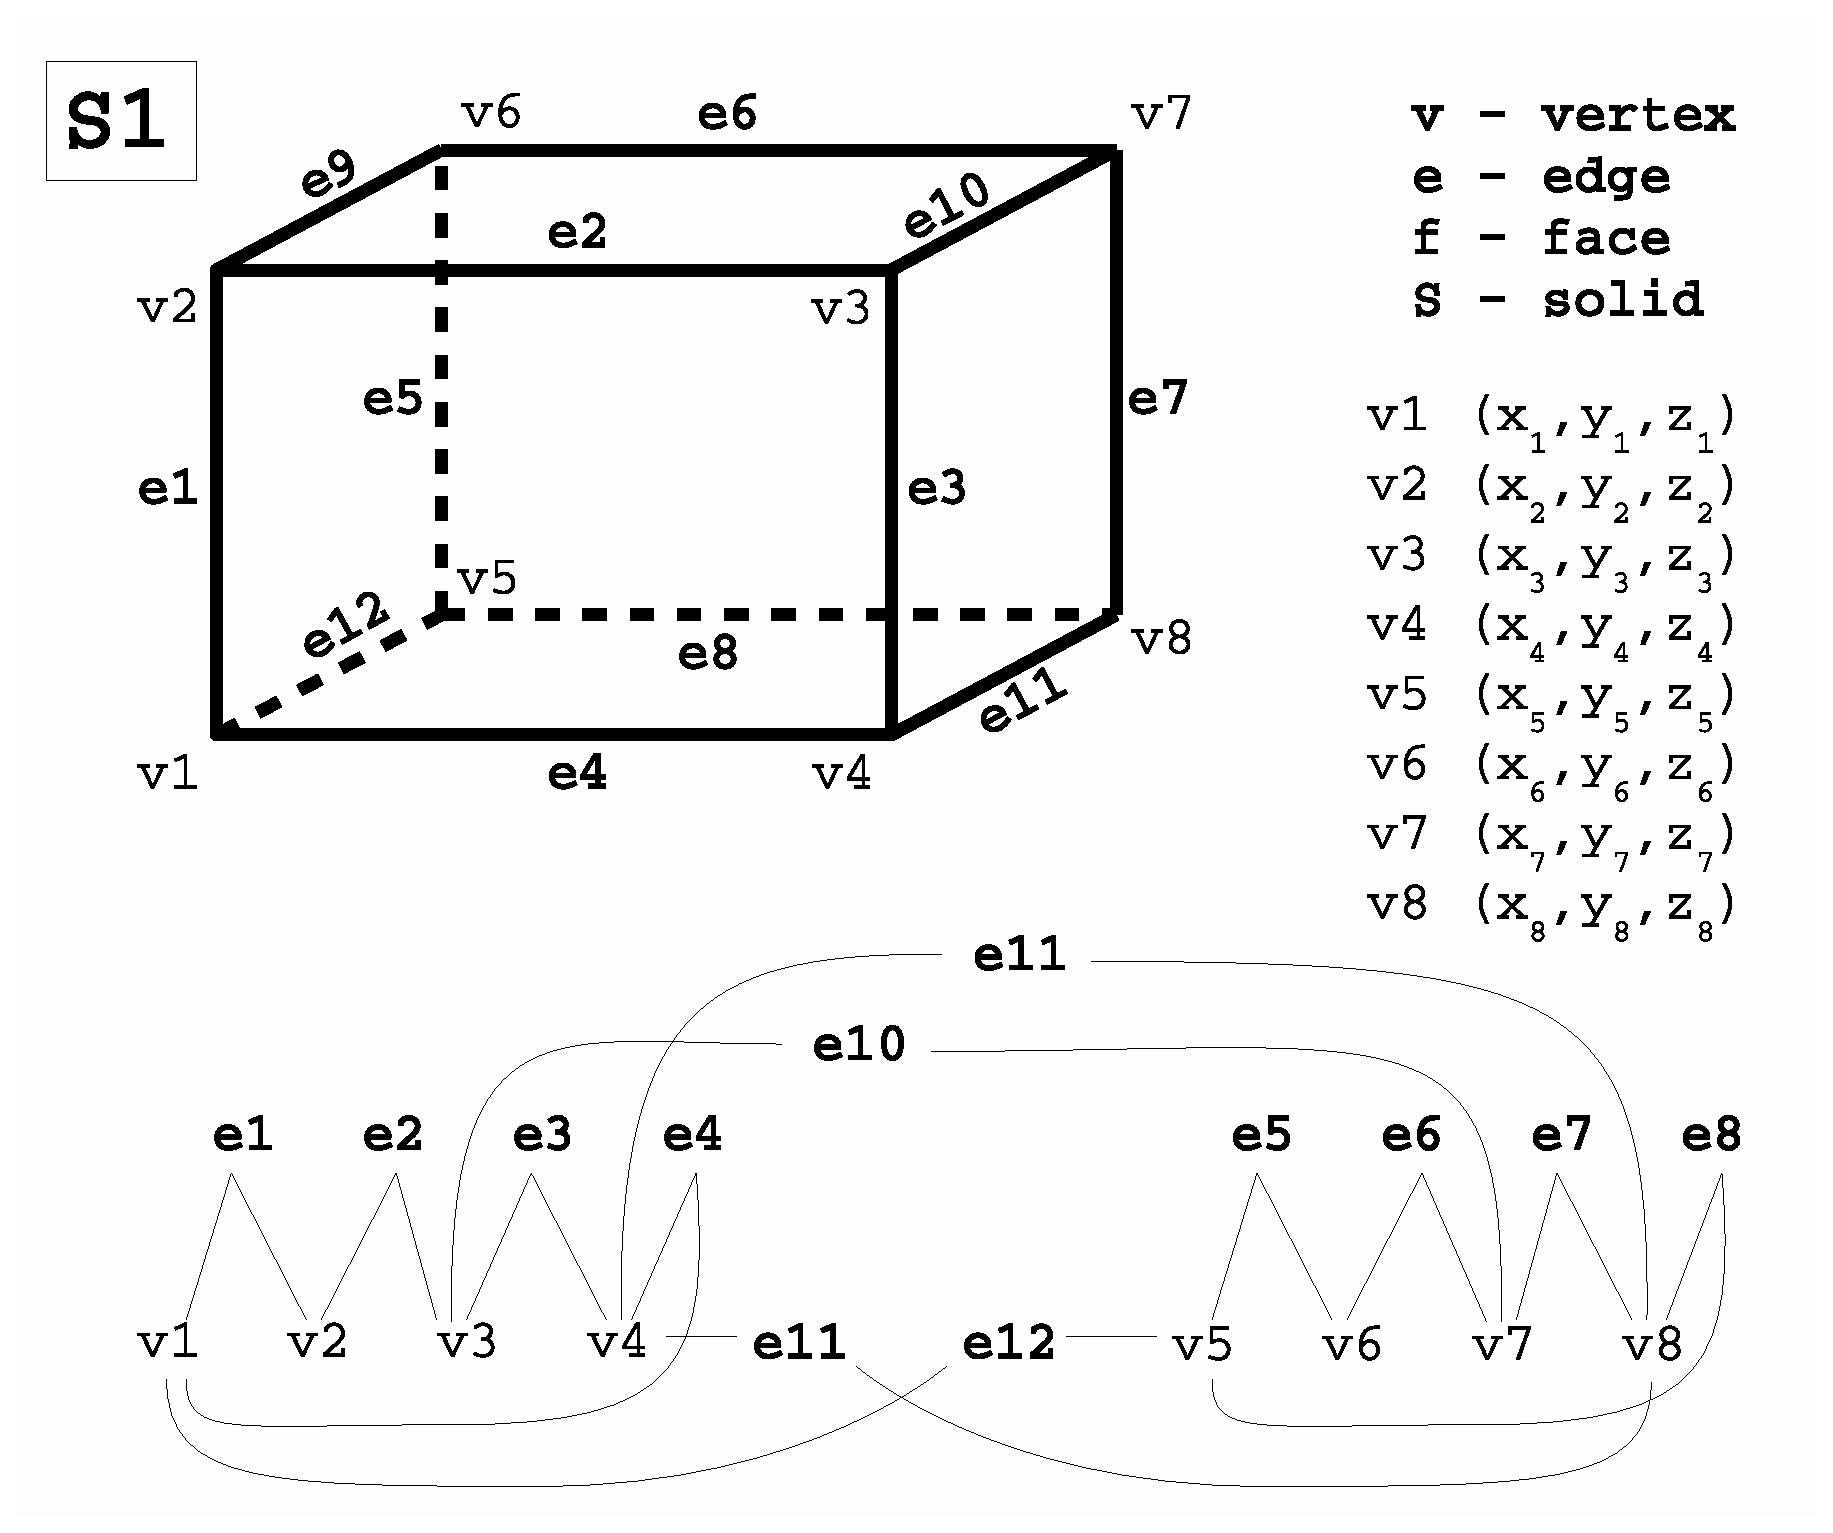
\includegraphics[width=0.7\textwidth]{pictures/BREPbox1.eps}
\caption{Описание вершин и рёбер примитива box методами BREP.}
\label{fig:BREPbox1}
\end{figure}

\begin{figure}[H]
\centering
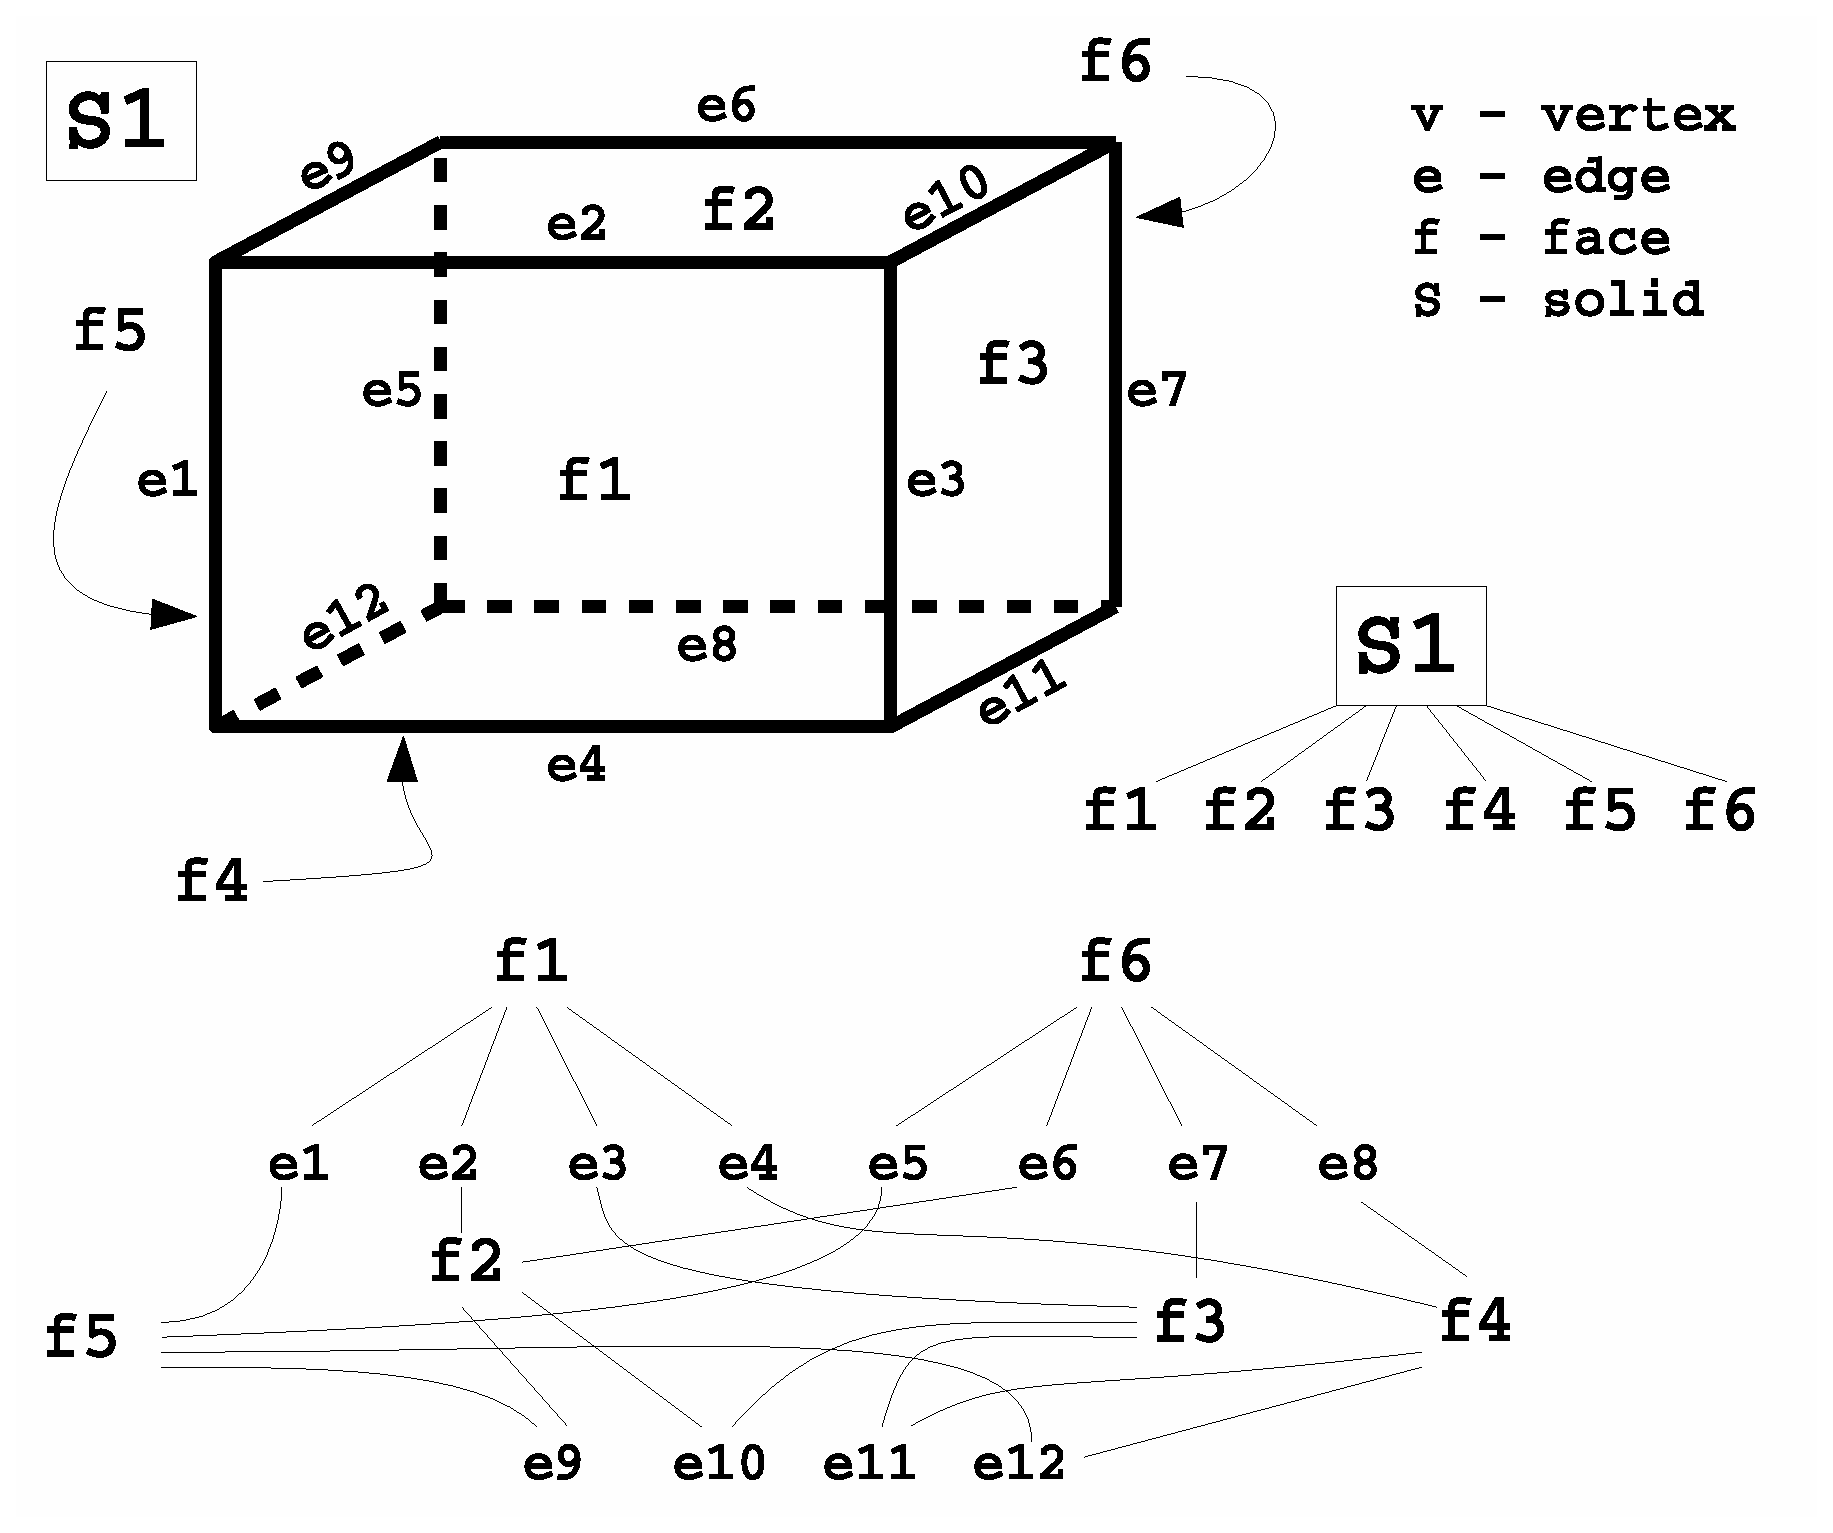
\includegraphics[width=0.7\textwidth]{pictures/BREPbox2.eps}
\caption{Описание граней и тела примитива box методами BREP.}
\label{fig:BREPbox2}
\end{figure}

%Подходы геометрического моделирования, принятые в САПР, обеспечивают максимально эффективную работу как ЭВМ, так и инженеров, в частности за счёт того, что эти подходы интуитивно понятны человеку.

Стоит, однако, отметить, что человек, создающий геометрическую модель в САПР, хотя и может выполнять построения в соответствии с базовыми принципами BREP, чаще всего применяет интуитивно понятные формообразования. Из последовательности этих формообразований система точно формирует BREP модель в памяти ЭВМ, которая также необходима для получения триангулированной геометрии для визуализации на дисплее ЭВМ~(\ref{sec:secGeoPoly}). Есть 4 базовых формообразования и 4 им обратных (с вычитанием) --- <<выдавливание>>, <<вращение>>, <<протягивание>> и <<тело по сечениям>>. Многие другие формообразования, такие как фаски и скругления, разрезы, отверстия, внутри на самом деле являются лишь вариациями перечисленных. Последовательность формообразований, выполненных пользователем для получения итоговой формы, сохраняется в виде дерева построения модели, напоминающего историю построения, но позволяющего навигацию и редактирование. Дерево часто доступно пользователю в основном рабочем окне интерфейса САПР. Однако бывают случаи, когда история построения теряется, например при передаче модели из одной САПР в другую. Таким образом, в результате работы инженера получается модель, описанная с помощью BREP, и во многих случаях имеющая также и дерево построения.

% \todo Пояснить, почему речь о CATIA.
% Ввёл чуть выше - в начале главы.

В инженерной практике принято проектировать и соответственно строить 3d-модели, объединяя в сборки детали и другие сборки. Отсюда вытекает, что во многих САПР, в том числе в CATIA~v5, существуют стандартные объекты, обозначающие детали и сборки. Например в САПР CATIA~v5 существует отдельный тип документа CATPart для детали и отдельный тип документа CATProduct для сборки. Внутри документа типа CATPart есть минимальный набор обязательных элементов --- 3 стандартные взаимноперпендикулярные плоскости в начале системы координат детали и главное тело детали, по умолчанию называемое PartBody. В документе типа CATProduct присутствует возможность добавлять в качестве дочерних компонентов либо документы CATPart либо другие документы CATProduct. В~\ref{sec:secBuilder} описывается, как соотносятся перечисленные сущности CATIA~v5 с понятиями геометрической подсистемы GEANT/ROOT.

Во многих САПР, в том числе и CATIA~v5 присутствует возможность так называемого контекстного редактирования компонентов. Это означает, что пользователь во время работы над сборкой в документе типа CATProduct, имеющей в качестве дочерних компонентов детали в файлах типа CATPart, может также редактировать эти детали, не переключая активный документ. Эта возможность широко используется в ``CATIA-GDML geometry builder'' --- большая часть работы выполняется в контексте единственного продукта, что с точки зрения пользователя аналогично работе над всей экспериментальной установкой.

%\todo
%Описать только нормальное применение BREP, то есть для замкнутых солидов.
BREP разрабатывался как наиболее общий метод представления геометрии в ЭВМ и не ограничивается описанием твёрдых тел. Отдельные поверхности, например, также являются корректными сущностями.

%Более того, возможна также некоторая корректировка подходов САПР к геометрическому моделированию с целью повышения совместимости с пакетами проведения частиц. \textbf{Один из возможных подходов --- реализация полигонального (см. секцию~\ref{sec:secGeoPoly}) твердотельного моделирования со строгим ограничением замкнутости оболочек, представляющих границы тела.} Однако следует учитывать следующие факты, мешающие движению в данном направлении. Во-первых, САПР --- это в большинстве своём коммерческое программное обеспечение с закрытым исходным кодом, а геометрическое ядро САПР --- базовая составляющая, которую отлаживают десятилетиями. Внесение изменений в столь важную компоненту коммерческого продукта, вероятно, будет проблемным даже при наличии интереса со стороны фирмы-разработчика. Во-вторых, в обеих сферах накоплен огромный массив моделей, применяемых для поддержки изделий на всех этапах жизненного цикла, даже после окончания процесса проектирования. GEANT/ROOT модели могут применяться для выполнения моделирования даже после того, как физическая экспериментальная установка уже собрана, а иногда даже и уже разобрана.

% ================================================================================================================
%   ____ ____   ____                                     _              
%  / ___/ ___| / ___|     __ _  ___  ___  _ __ ___   ___| |_ _ __ _   _ 
% | |   \___ \| |  _     / _` |/ _ \/ _ \| '_ ` _ \ / _ \ __| '__| | | |
% | |___ ___) | |_| |   | (_| |  __/ (_) | | | | | |  __/ |_| |  | |_| |
%  \____|____/ \____|    \__, |\___|\___/|_| |_| |_|\___|\__|_|   \__, |
%                        |___/                                    |___/ 
% ================================================================================================================

\subsection{Конструктивная твердотельная геометрия CSG}\label{sec:secGeoCSG}

Конструктивная твердотельная геометрия (Constructive Solid Geometry, CSG) --- один из способов описания геометрии в ЭВМ, в котором твёрдое тело (``solid'') представляет собой примитив либо результат Булевой операции над другими твёрдыми телами.

Изначально CSG использовался как основной способ представления геометрии в САПР, но по мере развития последних от CSG перешли к BREP. При этом, всё же, во многих САПР осталась возможность создавать CSG геометрию. CSG до сих пор активно применяется в некоторых узкоспециализированных областях --- например для описания экспериментальных установок для выполнения моделирования взаимодействия частиц с материалом (см.~\ref{sec:secGeoROOT}), для описания ячейки периодичности композитных материалов и др.

В качестве строительных блоков в CSG используются примитивы из списка реализованных в системе. Список примитивов обычно включает в себя как относительно простые примитивы типа параллелипипеда (box), сегмента цилиндра (tubs), сегмента конуса (cons), так и достаточно сложные, типа эллипсоида, параболоида, скрученных (twisted) примитивов.
Форма может быть описана либо как примитив, либо как результат Булевой операции над примитивами или другими Булевыми операциями.
Определено три Булевы операции (приведены оригинальные названия в GEANT/ROOT и соответствующие названия в CATIA~v5):

\begin{itemize}
\itemsep0pt
\item{Объединение (Union, Add);}
\item{Вычитание (Subtraction, Remove);}
\item{Пересечение (Intersection, Intersect).}
\end{itemize}

\begin{figure}[H]
\centering
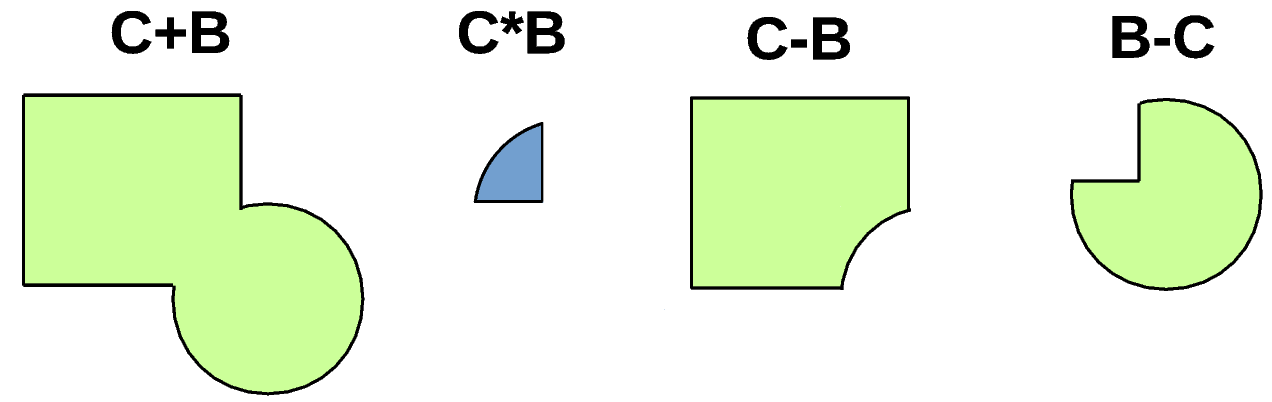
\includegraphics[width=0.6\textwidth]{pictures/Boolean.png}
\caption{Булевы операции.}
\label{fig:Boolean}
\end{figure}

Булевы операции не изменяют уравнений повехностей границ примитивов, а лишь могут сгенерировать новые рёбра на пересечениях граней примитивов. За счёт этого Булевы операции позволяют задать практически любую геометрическую форму, имеющую границы из тех, что применяются в примитивах.

% ================================================================================================================
%  ____       _                               _                                     _              
% |  _ \ ___ | |_   _  __ _  ___  _ __   __ _| |     __ _  ___  ___  _ __ ___   ___| |_ _ __ _   _ 
% | |_) / _ \| | | | |/ _` |/ _ \| '_ \ / _` | |    / _` |/ _ \/ _ \| '_ ` _ \ / _ \ __| '__| | | |
% |  __/ (_) | | |_| | (_| | (_) | | | | (_| | |   | (_| |  __/ (_) | | | | | |  __/ |_| |  | |_| |
% |_|   \___/|_|\__, |\__, |\___/|_| |_|\__,_|_|    \__, |\___|\___/|_| |_| |_|\___|\__|_|   \__, |
%               |___/ |___/                         |___/                                    |___/ 
% ================================================================================================================

\subsection{Полигональное геометрическое представление}\label{sec:secGeoPoly}

% в общем случае - запятые?
Полигональное (тесселированное, фасеточное) представление не менее распростанено, но имеет совершенно другую область применения. Строительным элементом полигональных моделей, в общем случае, является плоский многоугольник, называемый полигоном (polygon, pgon) или фасеткой (facet). Несколько таких многоугольников может стыковаться по рёбрам или вершинам, образуя поверхность, возможно описывающую границы некоторого объекта. Из этого следует, что, строго говоря, полигональное представление является частным случаем BREP с некоторыми допущениями, однако принято рассматривать его как отдельный способ по нескольким причинам.

% Слишком длинное предложение. Надо бы разбить.
В отличии от моделей, предназначенных для таких приложений как моделирование прохождения частиц через вещество или моделирование с помощью МКЭ (например, задач напряжённо-деформированного состояния), где для каждого тела обязательно должны быть определены его границы, отделяющие материал этого тела от окружающего пространства, объект полигональной модели в общем случае не обязан быть замкнутым. Это означает, что, в принципе, между полигонами могут быть зазоры. Это объясняется тем, что полигональные модели изначально рассчитаны на быструю визуализацию, а не выполнение над ними каких-либо расчётов.

Полигональная геометрия в основном применяется в мультипликации, для получения фотореалистичных изображений. При этом основное внимание уделяется не математически точному описанию границ поверхностей, а реалистичности или художественности визуализации модели на дисплее.
%В общем случае такая модель не требует наличия замкнутой оболочки для задания тела, допускается даже остсутствие части границ, если это не влияет на изображение на экране.
Для создания и удобного редактирования полигональных моделей применяется соответствующее ПО: Autodesk 3ds Max, Autodesk Maya, Blender и др.

Частный случай полигонального представления --- триангулированное представление --- имеет треугольники в качестве полигонов. Оно представляет особый интерес т.к. всегда строится для визуализизации на дисплее графической подсистемой того или иного пакета моделирования, даже если пользователь создаёт BREP или CSG. Главная причина для этого заключается в том, что триангулированные модели могут очень быстро обрабатываться 3D-конвейером графического адаптера ПК, как наиболее важный частный случай --- визуализироваться на дисплее.

% http://elanina.narod.ru/lanina/ind/graph/file103.htm

Большинство приложений трёхмерной графики, в том числе САПР, при построении объёмных сцен придерживаются определенной последо­вательности действий, в совокупности составляющей так называемый ЗD-конвейер. В качестве входных данных 3D-конвейер принимает массив треугольников, а итогом работы ЗD-конвейера является отрисовка (рендеринг) резуль­тирующего изображения на дисплее компьютера. Графический адаптер реализует аппаратное ускорение 3D-конвейера.

Несмотря на то что графический адаптер оптимизирован для обработки треугольников, существует ограничение на размер модели, определяемой доступной памятью (как ЦПУ, так и ГПУ). Также объём геометрической модели определяет время её обработки, например, выполнения матричных преобразований при изменении ракурса камеры. Это определяет частоту обновления изображения на дисплее, падение которой ниже некоторого уровня (\todo скажем, 20) сильно усложняет работу.
%Аналогично, увеличение количества элементов в КЭ-модели приводит к увеличению времени расчётов МКЭ.

%OpenGL (Open Graphics Library) --- спецификация, определяющая платформонезависимый (независимый от языка программирования) программный интерфейс для написания приложений, использующих двумерную и трёхмерную компьютерную графику. OpenGL де-факто является стандартом для всех трёхмерных приложений, его конвейер представлен на~\figref{fig:OGLpipeline}.

%\begin{figure}[H]
%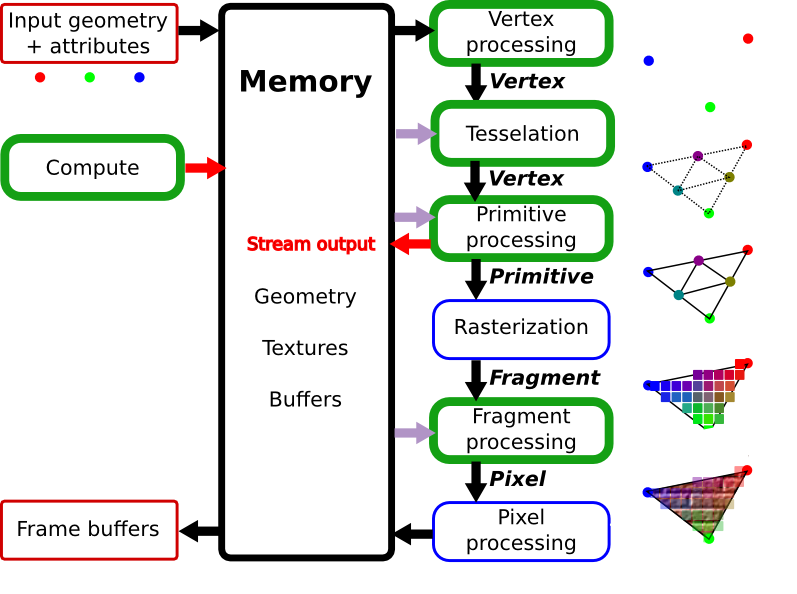
\includegraphics[width=0.8\textwidth]{pictures/pipeline-v4.png}
%\caption{Упрощённый конвейер OpenGL. На вход поступают координаты вершин и тройки индексов вершин, образующие треугольник. Выходной результат --- растровое (пиксельное) изображение, пригодное для отображения на дисплее.}
%\label{fig:OGLpipeline}
%\end{figure}

В промышленном геометрическом моделировании триангулированная геометрия применяется не только для визуализации. Например в стереолитографии, и вообще прототипировании, получил распространение формат обмена триангулированной геометрией STL, представляющий собой текстовый файл, в котором перечислены треугольники как группы по три вершины, а вершина задаётся тройкой координат (см. секцию~\ref{sec:secGeoFormats}).

% ================================================================================================================
%  _____ _____ __  __                                     _              
% |  ___| ____|  \/  |     __ _  ___  ___  _ __ ___   ___| |_ _ __ _   _ 
% | |_  |  _| | |\/| |    / _` |/ _ \/ _ \| '_ ` _ \ / _ \ __| '__| | | |
% |  _| | |___| |  | |   | (_| |  __/ (_) | | | | | |  __/ |_| |  | |_| |
% |_|   |_____|_|  |_|    \__, |\___|\___/|_| |_| |_|\___|\__|_|   \__, |
%                         |___/                                    |___/ 
% ================================================================================================================

\subsection{Конечно-элементное (КЭ) геометрическое представление}\label{sec:secGeoFEM}

В инженерной практике широкое распространение получил метод конечных элементов (МКЭ) --- численный метод решения дифференциальных уравнений с частными производными, а также интегральных уравнений, возникающих при решении задач прикладной физики. Метод широко используется для решения задач механики деформируемого твёрдого тела, динамики жидкостей и газов, теплообмена, электродинамики и т.д. МКЭ, как и некоторые другие численные методы, требует геометрическую модель в качестве входных данных.

Метод конечных элементов получил своё название от способа разбиения расчётной области на элементарные блоки --- конечные элементы (КЭ). Строго говоря, КЭ --- это не только геометрическая форма, но и модель аппроксимации решения внутри области, ограниченной этой формой. Существует огромное множество типов КЭ, причём существуют элементы имеющие одинаковую геометрию, но разные математические модели. Расчётная область может быть разбита на элементы различных типов. Исходя из условий решаемой задачи инженер-расчётчик выбирает, какими элементами разбивать расчётную область, а также, обычно, задаёт какие-либо указания модулю разбиения геометрии на сетку в расчётном программном обеспечении. В простом случае расчётной областью является пространство заполненное материалом, т.е. сама деталь, а конечным элементом --- тетраэдр. Модель, в которой деталь представлена множеством КЭ, соответственно называют КЭ-моделью.
% Вырезан кусок... Ушёл в обмен геометриями

% ================================================================================================================
%   ____                                 _                 
%  / ___|___  _ __ ___  _ __   __ _ _ __(_)___  ___  _ __  
% | |   / _ \| '_ ` _ \| '_ \ / _` | '__| / __|/ _ \| '_ \ 
% | |__| (_) | | | | | | |_) | (_| | |  | \__ \ (_) | | | |
%  \____\___/|_| |_| |_| .__/ \__,_|_|  |_|___/\___/|_| |_|
%                      |_|                                 
% ================================================================================================================

\section{Сравнение CSG, BREP и полигональных моделей}

На~\figref{fig:DiffGeoRepr} показана одна и та же геометрическая форма, описанная в ЭВМ с помощью различных методов представления геометрии.

На верхнем левом рисунке показаны отдельные примитивы до выполнения Булевой операции. Можно видеть кривые пересечения примитивов, однако фактически уравнения этих кривых на пересечении конкретных уравнений поверхностей либо не рассчитаны вообще, либо расчитаны системой моделирования неявно исключительно для более красивой визуализации.
На верхнем правом рисунке показано твёрдое тело после выполнения Булевой операции. Здесь рёбра на пересечениях уже явно рассчитаны.
На нижнем левом рисунке показана модель после выполнения Булевой операции, триангулированная системой моделирования для визуализации, в таком режиме, когда показываются только рёбра треугольников. Отметим, что именно в такой форме, но с закрашенными треугольниками, все модели, независимо от внутреннего описания --- BREP, CSG или какое-либо другое --- визуализируются на дисплее ЭВМ. За счёт того, что угол между рёбрами треугольников, аппроксимирующими гладкое ребро исходного тела, очень мал, визуально создаётся ощущение плавных кривых.
На нижнем правом рисунке показана КЭ-модель, полученная разбиением исходной BREP модели на тетраэдральные конечные элементы с помощью пакета Netgen~(\cite{NETGEN}). Видны только треугольники на поверхности, но на самом деле на тетраэдры разбито всё твёрдое тело.
Стоит отметить отличие триангуляции поверхностей для КЭ-модели и модели для визуализации. Это объясняется разными критериями алгоритма триангуляции в силу разных целей моделей.

\begin{figure}[H]
\begin{minipage}[b]{0.495\textwidth}
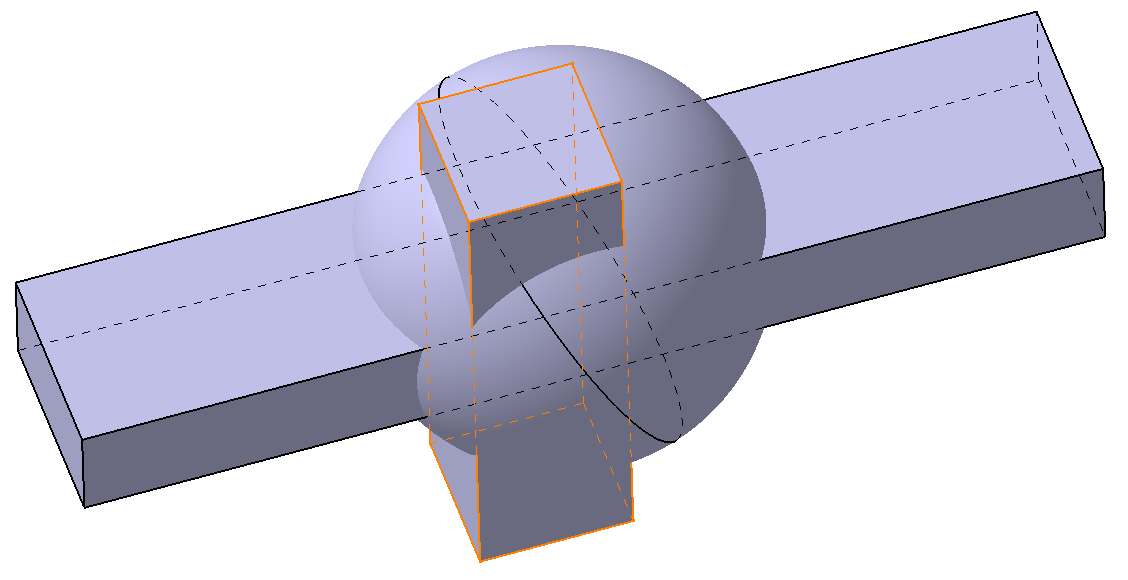
\includegraphics[width=1.0\textwidth]{pictures/Separate_primitives.png}
\end{minipage}
\hspace{0.01\textwidth}
\begin{minipage}[b]{0.495\textwidth}
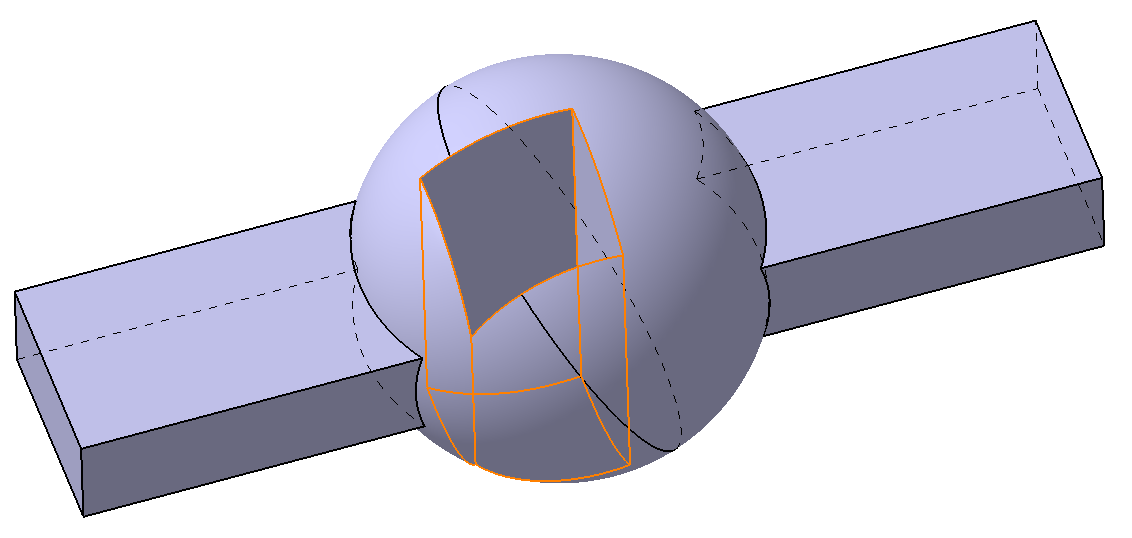
\includegraphics[width=1.0\textwidth]{pictures/BREP_2.png}
\end{minipage}
\begin{minipage}[b]{0.495\textwidth}
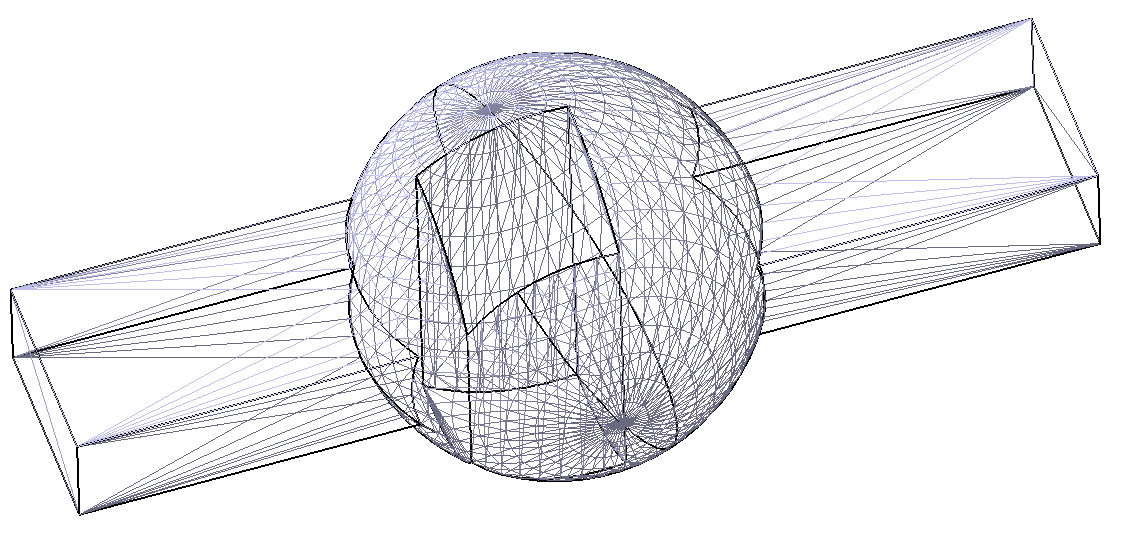
\includegraphics[width=1.0\textwidth]{pictures/Triangles.png}
\end{minipage}
\hspace{0.01\textwidth}
\begin{minipage}[b]{0.495\textwidth}
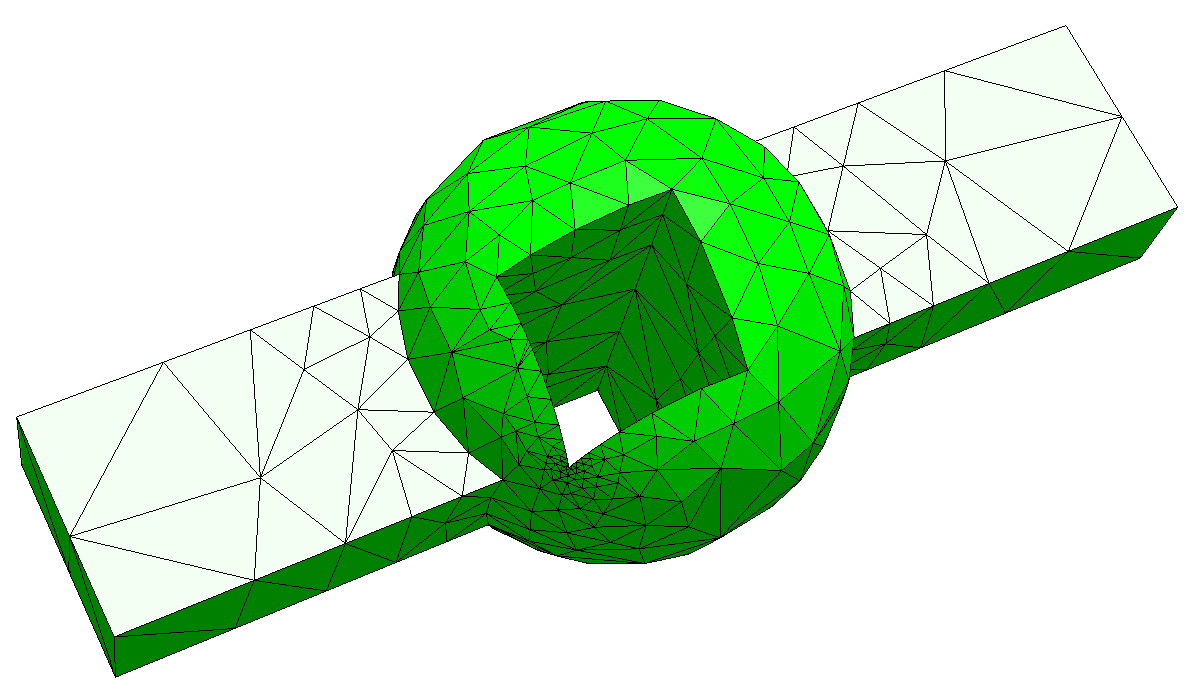
\includegraphics[width=1.0\textwidth]{pictures/FEM_rough.png}
\end{minipage}
\caption{Одна и та же геометрическая форма, описанная различными представлениями.}
\label{fig:DiffGeoRepr}
\end{figure}

% ================================================================================================================
%   ____                 __                            _       
%  / ___| ___  ___      / _| ___  _ __ _ __ ___   __ _| |_ ___ 
% | |  _ / _ \/ _ \    | |_ / _ \| '__| '_ ` _ \ / _` | __/ __|
% | |_| |  __/ (_) |   |  _| (_) | |  | | | | | | (_| | |_\__ \
%  \____|\___|\___/    |_|  \___/|_|  |_| |_| |_|\__,_|\__|___/
%                                                              
% ================================================================================================================

\subsection{Обмен геометрической информацией}\label{sec:secGeoFormats}

% \todo (например, BREP и триангулированная вместе в файле одного формата - ?)

Существует огромное множество форматов для обмена геометрией между различными программными продуктами. Следует различать геометрическое представление и формат, в котором данные записаны в файл. Существуют универсальные форматы, которые позволяют записывать в файл геометрию, представленную разными способами, но в большинстве случаев один формат подразумевает один способ представления геометрии. Данные могут быть записаны в файл как в виде текста, так и в бинарном виде. Проприетарные форматы в большинстве своём не имеют открытой спецификации, поэтому файлы этого формата бинарные, создаются и читаются ограниченным списком программ, в который, в первую очередь, входят продукты от фирм, являющихся авторами этих форматов. Также иногда эти фирмы дают возможность купить лицензию на модуль импорта/экспорта того или иного формата для реализации его поддержки в стороннем ПО.

Из множества популярных форматов для хранения и передачи геометрической информации, не подразумевающей перевод между различными представлениями, рассмотрим несколько наиболее употребимых в нашей области.

% \subsubsection{STEP}\label{sec:secSTEP}

ISO-10303 \textbf{STEP} (STandard for Exchange of Product model data) --- независимый стандарт, получивший наибольшее распространение в инженерной практике для обмена информацией об изделии, в том числе геометрическими моделями.
%В наши дни практически любая САПР имеет возможность импорта и экспорта STEP.
%Данный стандарт предоставляет широкие возможности по обмену информацией об изделии.
Особенностью данного стандарта является наличие большого количества инструментов для описания BREP-геометрии. В то же время, следует отметить, что несмотря на то, что практические все современные САПР используют идентичные подходы к моделированию и имеют поддержку данного формата, STEP файлы не хранят дерево построения модели. По этой причине, даже если экспортировать STEP-файл из некоторой системы и импортировать обратно, то дерево построения, то есть последовательность формообразований, утеряется.
Обменные файлы STEP являются текстовыми. С одной стороны, это значительно упрощает разработку модулей для их импорта и экспорта, но с другой стороны, это приводит к тому, что для крупных моделей размер STEP-файлов становится достаточно большим, а следовательно и растёт время их обработки.

% \subsubsection{IGES}\label{sec:secIGES}

\textbf{IGES} (Initial Graphics Exchange Specification) --- независимый стандартизированный формат для обмена информацией между САПР, включая геометрические модели. В настоящее время многие САПР имеют поддержку IGES, однако данный формат можно рассматривать как устаревший, практически вытесненный стандартом STEP.

% \subsubsection{STL}\label{sec:secSTL}

\textbf{STL} (STereoLithography) --- текстовый формат для обмена тесселированной геометрией, который, возможно, является самым распространённым на данный момент форматом для передачи моделей в сфере 3d-сканирования и 3d-печати.

% \subsubsection{OBJ}\label{sec:secOBJ}

\textbf{OBJ} --- очень простой и открытый текстовый формат для обмена полигональными моделями. В файл OBJ записаны координаты вершин, списки индексов вершин каждого полигона и некоторые вспомогательные данные, типа текстурных координат и др.

% \subsubsection{CGR}\label{sec:secCGR}

% http://www.datakit.com/en/news/who-or-what-is-cgr--92.html

\textbf{CGR} (Catia Graphical Representation) --- проприетарный формат Dassault Systemes, используемый для хранения триангулированной модели, готовой для быстрой визуализации на дисплее. Позволяет одновременно, в одном файле, хранить несколько моделей, что широко применяется для хранения нескольких уровней детализации.
% \todo проверить

% \subsubsection{3DXML}\label{sec:sec3dXML}

%\textbf{3DXML} --- проприетарный формат Dassault Systemes, используемый для хранения триангулированной модели, готовой для быстрой визуализации на дисплее. 3DXML имеет закрытую спецификацию. Файл этого формата представляет собой архив с одним или несколькими геометрическими моделями и дополнительной информацией. 3DXML player --- это бесплатный продукт Dassault Systemes, позволяющий просматривать модели в файлах 3DXML.

% \subsubsection{VRML, WRL, X3D}\label{sec:secVRML}

%\textbf{VRML} (Virtual Reality Modeling Language). Файлы формата VRML имеют расширение wrl. \textbf{X3D} --- стандартизированный (ISO/IEC 19775/19776/19777) формат, являющийся наследником VRML.

% \subsubsection{COLLADA}\label{sec:secCOLLADA}

% https://www.iso.org/standard/59902.html
% https://en.wikipedia.org/wiki/COLLADA
% https://www.khronos.org/collada/

%Основанный на XML формат \textbf{COLLADA} (COLLAborative Design Activity) разработан специально для обмена геометрической информацией между интерактивными приложениями, такими как игровые движки, различные системы полигонального моделирования, САПР, и т.д. Файлы формата COLLADA имеют расширение dae (digital asset exchange). Формат COLLADA поддерживается некоммерческой организацией Khronos group, а в 2013 году был опубликован как международный стандарт ISO/PAS 17506:2012.

% \subsubsection{NEU, ANEU}\label{sec:secNEU}
% Простой текстовый формат для задания ...

% ================================================================================================================
%     _         _                                               _             
%    / \  _   _| |_ ___        ___ ___  _ ____   _____ _ __ ___(_) ___  _ __  
%   / _ \| | | | __/ _ \      / __/ _ \| '_ \ \ / / _ \ '__/ __| |/ _ \| '_ \ 
%  / ___ \ |_| | || (_) |    | (_| (_) | | | \ V /  __/ |  \__ \ | (_) | | | |
% /_/   \_\__,_|\__\___(_)    \___\___/|_| |_|\_/ \___|_|  |___/_|\___/|_| |_|
%                                                                             
% ================================================================================================================

\subsection{Возможности автоматического перевода между способами представления}\label{sec:secAutoConversion}

%Существует теоретическая возможность прямой конвертации из представления, принятого в GEANT/ROOT, в BREP, однако в процессе работы не было найдено существующей реализации подобного перехода. Конвертация в обратном направлении до настоящего времени не была математически описана, хотя теоретически также представляется возможной.

\subsubsection{Конвертация CSG в BREP}\label{sec:secCSGtoBREP}

Поверхности, используемые в качестве границ примитивов CSG --- это чаще всего поверхности, описываемые относительно простыми уравнениями; большая часть из них --- уравнения первого и второго порядка. Очевидно, что перевод отдельных примитивов в BREP-описание не представляет сложности независимо от вида уравнений, описывающих их границы --- для этого не требуется никаких дополнительных вычислений. Чуть более сложная задача, но всё же полность решённая, --- автоматический перевод формы, полученной в результате Булевой операции, в BREP-описание. В случае Булевой операции в CSG нет явного описания рёбер и вершин, полученных в результате пересечения отдельных граней примитивов, однако эти рёбра вершины напрямую получаются из параметров операндов и их позиционирования. Таким образом возможна быстрая и полностью автоматическая конвертация CSG-модели в BREP, и она реализована, возможно в неявном виде, во всех САПР.

Полная --- значит абсолютно все примитивы могут быть описаны с помощью BREP.

\subsubsection{Конвертация BREP в Polygonal}\label{sec:secBREPtoPolygonal}

Суть получения полигональной геометрии из полноценного BREP описания заключается в аппроксимации всех граней набором плоских фасеток. Очевидно, что если исходная грань не плоская, то аппроксиммирующая полиногальная сетка будет иметь от неё некоторое отклонение.
Давно разработаны и хорошо отлажены алгоритмы для такой аппроксимации. Точность аппроксимации --- управляющий параметр процедуры. Для более точной аппроксимации требуется больше полиногов, а следовательно возрастает нагрузка на графический адаптер.

Многие из них основаны на триангуляции Делоне, разработанной в начале 20~века.

Таким образом возможна полная и \todo беспроблемная \todo конвертация BREP-модели в полигональную, и она реализована, возможно в неявном виде, во всех САПР.

Полная --- значит абсолютно все примитивы BREP (точки, рёбра, грани) могут быть приблизительно, с заданной точностью, описаны полигональной сеткой. Управляющий параметр --- точность аппроксимации.

\subsubsection{Конвертация BREP в FEM}\label{sec:secBREPtoFEM}

Существуют алгоритмы, позволяющие эффективно получить разбиение исходной геометрической модели, например представленной с помощью BREP и построенной в САПР, на конечные элементы. Из того что возможен автоматический перевод из CSG в BREP вытекает, что возможен также и перевод из CSG в КЭ-модель.

Первый этап процедуры разбиения твёрдого тела на конечные элементы заключается в триангуляции и выполняется теми же алгоритмами, что и для получения полиногальных моделей из BREP. Затем на основе разбиения граней строится пространственная сетка.
При этом инженер обычно глазами смотрит на сетку. Также при разбиении на сетку расчётчик руками даёт указания алгоритму. Например, на сколько элементов разбить то или иное ребро. Критерий построенной --- кривота элементов. Процедура разбиения тела на КЭ сложна и для более-менее сложной детали выполняется в несколько итераций. 

\subsubsection{Конвертация из BREP в CSG}\label{sec:secBREPtoCSG}

Если тело (solid) представляет собой примитив, описанный средствами BREP (см. секцию~\ref{sec:geoCAD}), то представляется возможным реализовать алгоритм, распознающий этот факт и определяющий параметры примитива. Сначала необходимо выполнить проверку топологии тела (тело ограничено шестью плоскими гранями, стыкующимися по 12 рёбрам, и т.д.), затем выполнить геометрические проверки (перпендикурярность плоскостей, углы между рёбрами и т.д.). Задача усложнена тем, что за счёт богатых возможностей BREP фактически правильная фигура может быть описана бесконечным количеством способов. Можно привести следующий простой пример. Плоская прямоугольная грань может быть описана уравнением плоскости и замкнутым циклом из 4-х взаимноперпендикулярных рёбер (прямоугольник) на этой плоскости, а может быть разбита на два треугольника на той же плоскости, смежных по гипотенузе. Эти два описания обозначают геометрически эквивалентные формы, но во втором случае потребуется дополнительная процедура приведения двух треугольников к одному прямоугольнику --- суть, минимальному полному описанию.

Основной фактор, делающий невозможным полный перевод BREP-модели в CSG, заключается в том, что CSG имеет ограниченный список уравнений поверхностей, чаще всего не выше второго порядка, в то время как BREP позволяет задавать грани на основе поверхностей, описанных сложными уравнениями, например NURBS (\cite{NURBS}). Для описания таких сложных поверхностей можно прибегнуть к аппроксимации существующими в примитивах поверхностями. (\todo но это будет уже не полная конвертация)
Однако этот фактор является не главным, т.к. из практики известно, что подавляющее большинство геометрических форм в области детекторов --- достаточно простые.
Главная причина невозможности перевода из BREP в CSG заключается в том, что в подавляющем большинстве случаев форма тела не является примитивом. При переводе требуется каким-то образом представить её как результат Булевой операции.

% Описанные выше геометрические задачи также имеют следующую особенность. По причине ограниченности машинного слова числа с плавающей запятой хранятся в ПК с ограниченной точностью и выполнение расчётов, включающих матричные преобразования и тригонометрические функции, приводят к появлению заметных вычислительных ошибок. В большинстве случаев удаётся преодолеть эту проблему округлением до заданного знака, т.к. на практике в компьютерном геометрическом моделировании можно задаться физически обоснованным пределом снизу, например 1~мкм, или, с запасом, 1~нм, т.е. заведомо на много порядков выше точности вычислений. Но, к сожалению, это не всегда помогает.

% \subsubsection{Конвертация FEM в BREP}\label{sec:secFEMtoBREP}

% На практике не возникает необходимости переводить описание модели из КЭ в какое-либо другое. КЭ-модель всегда (кроме каких-то экстренных ситуаций) получена построением сетки на основе BREP или CSG. В КЭ-моделях границы тел описываются так же как и в полигональных. Следовательно, с теоретической точки зрения, перевод из FEM в BREP эквивалентен переводу из полигонального представления в BREP.

\subsubsection{Конвертация Polygonal в BREP}\label{sec:secPolyToBREP}

Если полиногами описана замкнутая оболочка, то представляется возможным объявить эту оболочку границой твёрдого тела, таким образом переведя без потерь полигональное описание в BREP, чтобы в дальнейшем работать средствами твердотельного моделирования. Если до цельности оболочки нехватает некоторого количества полигонов, то система обычно позволяет автоматически заполнить дыры плоскими фастеками, чтобы дальше можно было получить твёрдое тело.

% \todo Разобраться
Данная задача возникает при обработке результатов 3d-сканирования. 3d-сканеры выдают облако точек и первым этапом выполняется построение полиногальной модели по точкам. Затем обычно выполняется автоматизированное дополнение полинональной модели до замкнутой оболочки для получения твёрдого тела.

% Проблема имеет некоторое сходство с конвертацией CSG в BREP.

\textbf{Концентрируемся только на BREP, в котором описываются твёрдые тела, ограниченные замнутой оболочкой из поверхностей, либо большие непрерывные поверхности.}


% ================================================================================================================
%   ____ _____    _    _   _ _____  ______   ___   ___ _____                                     _              
%  / ___| ____|  / \  | \ | |_   _|/ /  _ \ / _ \ / _ \_   _|     __ _  ___  ___  _ __ ___   ___| |_ _ __ _   _ 
% | |  _|  _|   / _ \ |  \| | | | / /| |_) | | | | | | || |      / _` |/ _ \/ _ \| '_ ` _ \ / _ \ __| '__| | | |
% | |_| | |___ / ___ \| |\  | | |/ / |  _ <| |_| | |_| || |     | (_| |  __/ (_) | | | | | |  __/ |_| |  | |_| |
%  \____|_____/_/   \_\_| \_| |_/_/  |_| \_\\___/ \___/ |_|      \__, |\___|\___/|_| |_| |_|\___|\__|_|   \__, |
%                                                                |___/                                    |___/ 
% ================================================================================================================

\section{Представление геометрии в GEANT/ROOT}\label{sec:secGeoROOT}

Существует несколько способов задать геометрию для VMC-связки GEANT+ROOT --- с помощью текста (geo), с помощью XML в файле формата GDML, в виде макроса на языке ``C'', интерпретируемого системой ROOT и формирующего выходной файл (обычно --- .root, но возможно и .gdml). Также возможно использование какого-либо программного инструмента, некоторые из которых описаны в секции~\ref{sec:ExistSols}.

% \todo переформулировать
Список реализованных в GEANT4 и ROOT примитивов совпадает практически полностью. В настоящее время в рамках проекта AIDA (\cite{AIDA}) в ЦЕРН ведётся разработка пакета Unified Solids (\cite{USOLIDS}), ставящего своей задачей получить единое описание геометрии в пакетах GEANT4 и ROOT.

Для описания геометрических форм в пакетах GEANT/ROOT применяется CSG (см. секцию~\ref{sec:secGeoCSG}).
Алгоритмы проведения частиц, реализованные в GEANT/ROOT, оптимизированы для соответствующего описания геометрии, применяемого в этих пакетах.
Принимая во внимание тот факт, что геометрия в GEANT/ROOT нужна для выполнения моделирования взаимодействия частиц с материалом, можно сказать, что примитив --- это объект, имеющий геометрическое представление и для которого реализовано решение геометрических задач, возникающих при моделировании. Среди таких геометрических задач можно отметить задачу нахождения расстояния до ближайшей границы примитива от некоторой точки внутри объёма, в одном заданном направлении или в любом возможном направлении. Эту задачу необходимо решать многократно в процессе проведения частицы для того чтобы определить так называемый максимальный допустимый геометрический шаг. В результате моделирования физических процессов получается максимальный допустимый шаг из соображений физики. Для того чтобы собственно изменить координату частицы из этих двух шагов выбирается минимальный. Каждый примитив, как в GEANT4, так и в ROOT, реализован как отдельный C++ класс, имеющий свои геометрические параметры среди членов данных, и решение описанных выше геометрических задач среди методов. Следует, отметить, что есть только параметры примитива, но нет никакого описания типа BREP. Уравнения границ фигурируют лишь в неявном виде в коде методов для решения геометрических задач. Более подробно примитивы описаны в~\ref{sec:Primitives}.

% Перетащено из Boolean
При этом не требуется дополнительной реализации решения геометрических задач, т.к. удаётся комбинировать то, что реализовано в примитивах.
Особенности применения Булевых операций для задания формы объёма в ``CATIA-GDML geometry builder'' описано в~\ref{sec:Boolean}.

%Таким образом
Наблюдается некоторая аналогия между BREP и CSG, заключающаяся в том, что в любом случае сложное тело или базовый примитив имеет некоторые границы, заданные аналитическими выражениями. Корни этой аналогии лежат в фундаментальной математике. Однако решающая разница заключается в том, что для примитива эти границы чётко определены и имеется лишь ограниченное число параметров, позволяющих изменять форму примитива.

% А первая --- это форма с помощью CSG, если чё.
Вторая составляющая геометрического представления в GEANT/ROOT это иерархия объёмов.
Введём понятия логического и физического объёмов, формы и материала. Логический объём (logical volume), или просто объём (volume) это базовый элемент для построения иерархии объёмов. Объём описывает непозиционированный объект и всё, что находится внутри него. Объём характеризуется формой (shape) и материалом (material). Форма --- это заданные с помощью CSG границы пространства, по методу, описанному выше. Материал включает в себя описание химического состава, плотности, и т.д. При помещении одного логического объёма в другой, например объёма $A$ в объём $B$, образуется так называемый физический объём (physical volume), или узел (node), $B_1$, который обозначает взаимоотношение $A$ и $B$ как материнский-дочерний и характеризуется некоторой матрицей $M_{B1A}$ позиционирования $B_1$ внутри $A$.

\begin{figure}[H]
\centering
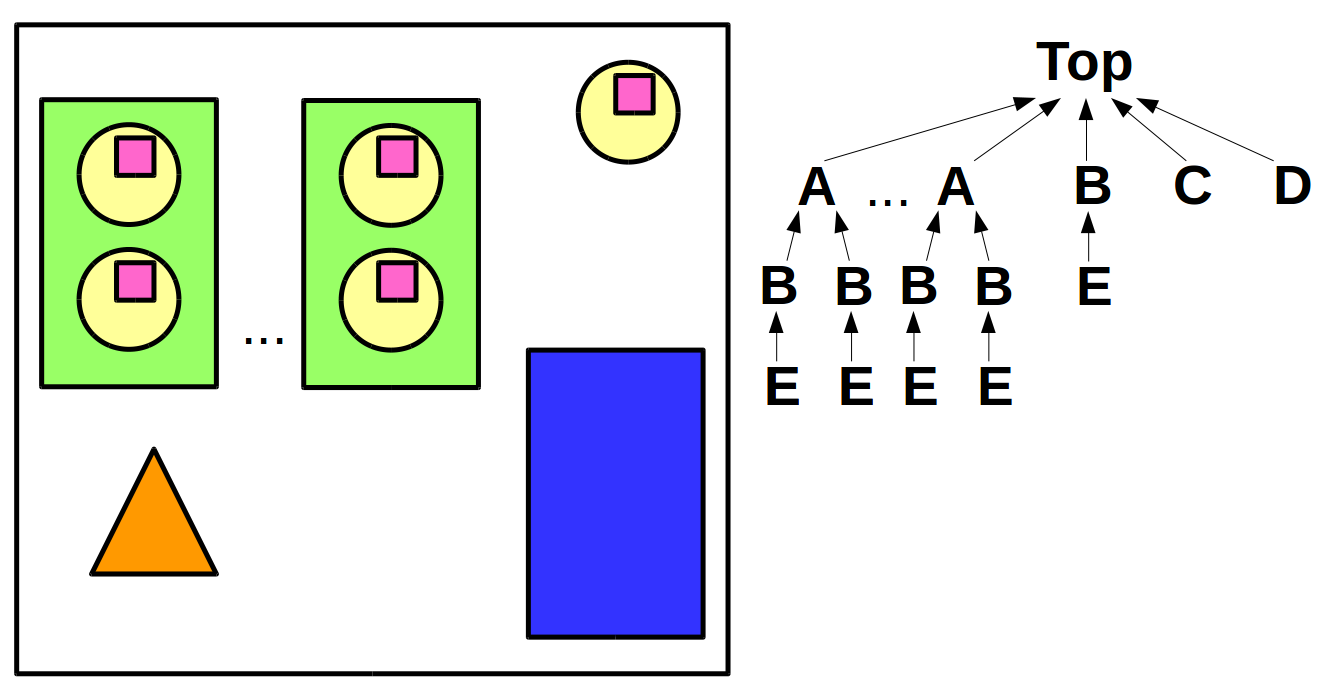
\includegraphics[width=0.7\textwidth]{pictures/ROOT_geo1.png}
\caption{Пример MC-геометрии, цвет означает материал. Полное дерево MC-модели (справа). Хранение такого полного описания геометрии невозможно из-за ограничения по памяти, однако часть дерева строится динамически по мере проведения частицы через геометрию.} % \todo
\label{fig:ROOTgeo1}
\end{figure}

\begin{figure}[H]
\centering
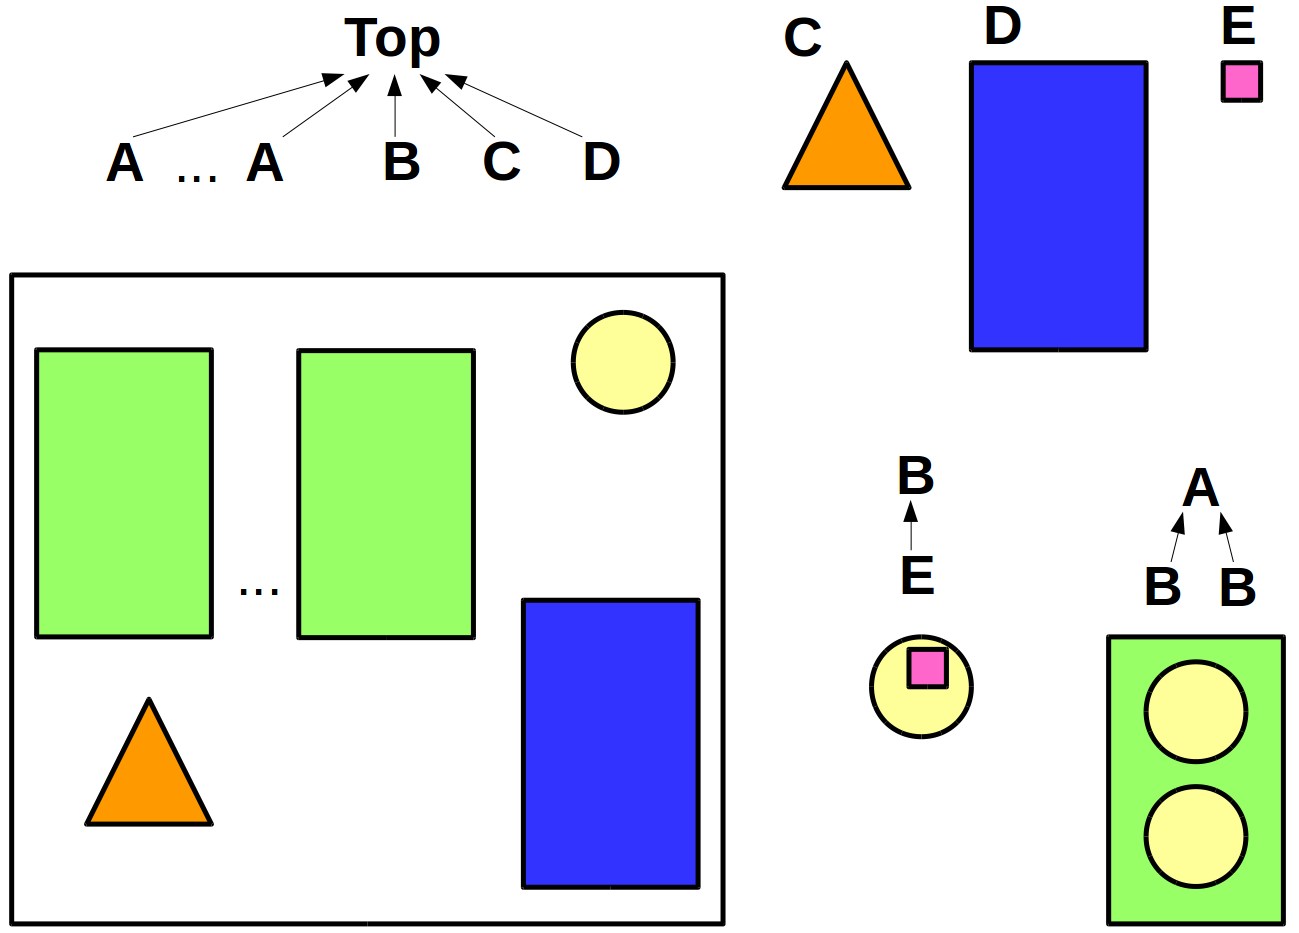
\includegraphics[width=0.7\textwidth]{pictures/ROOT_geo2.png}
\caption{Пример MC-геометрии, цвет означает материал. Более компактное эквивалентное описание той же геометрии, которое используется в системах проведения частиц ROOT и GEANT4. Сохраняются только локальные под-деревья --- взаимоотношения материнский-дочерний для одного уровня.} % \todo
\label{fig:ROOTgeo2}
\end{figure}

\begin{figure}[H]
\centering
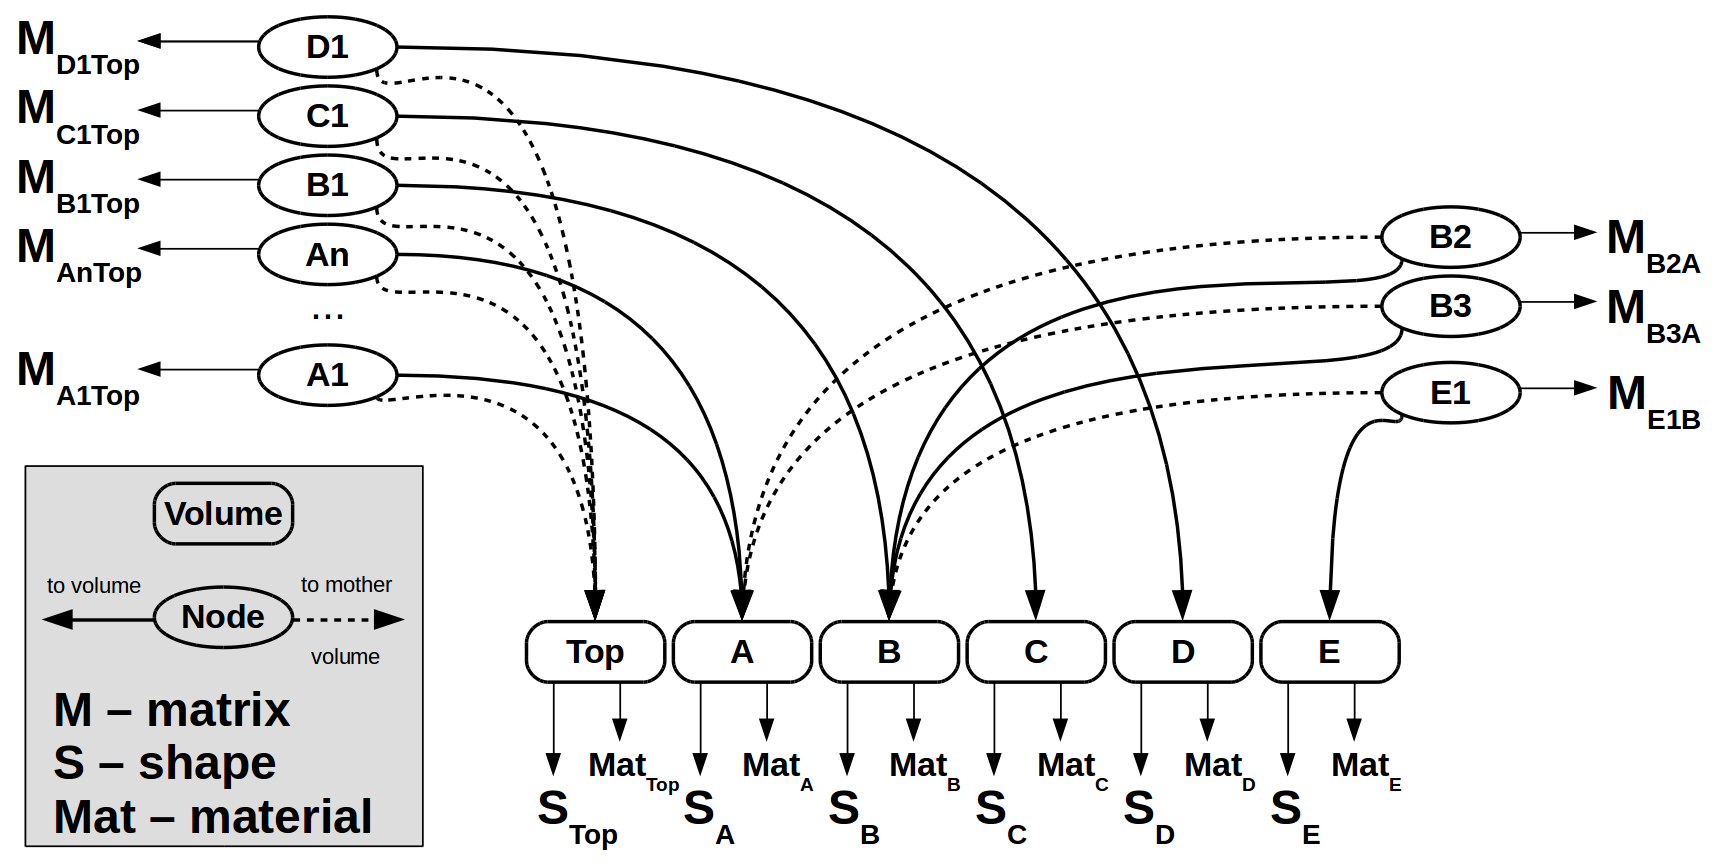
\includegraphics[width=0.7\textwidth]{pictures/ROOT_geo3.png}
\caption{ Эквивалентное представление данной геометрии с помощью объектов классов TGeo* в памяти ЭВМ. Стрелки обозначают указатели.} % \todo
\label{fig:ROOTgeo3}
\end{figure}

Принимая во внимание развитие вычислительной техники, в особенности резкое повышение производительности графических карт, их доступность широким массам, и вообще увеличение их значимости в вычислениях общего назначения, представляется возможным разработка новых алгоритмов проведения частиц через материал, учитывающих особенности геометрического представления в САПР.

Чем выше уровень подробностей в геометрической модели, применяемой для моделирования с помощью GEANT/ROOT, тем больше времени занимает это моделирование. Для оценочных расчётов удобно применять грубые модели, для точного определения каких-либо характеристик --- подробные модели. Поэтому принято иметь несколько MC-моделей одной и той же установки, имеющих разный уровень подробностей.
% упомянуть FastMC ?
В САПР подобная проблема решается другим образом. Так, например, в САПР CATIA~v5 присутствует возможность автоматического огрубления геометрической модели для снижения нагрузки на графический адаптер и повышения частоты кадров при динамической визуализации трёхмерных объектов. Это становится актуально, когда количество треугольников, которые необходимо визуализировать, составляет десятки миллионов.

% Asssembly-volume
\subsection{Assembly-volume}\label{sec:secAssemblyVolume}

В GEANT/ROOT существует тип объёмов, называемый Assembly, который характеризуется тем, что он не имеет формы и материала. Практически объём типа Assembly является контейнером без границ, который объединяет свои дочерние объёмы, что особенно удобно как минимум в двух случаях. Во-первых, если необходимо многократно позиционировать группу объёмов, которую невозможно охватить простой формой. Во-вторых, если преобразование координат при позиционировании одного или группы объёмов имеет сложную структуру и удобно представить его как суперпозицию двух преобразований.
%Как частный случай можно упомянуть ситуацию, когда какой-либо параметр преобразования является параметром модели (см. секцию~\ref{sec:Parameterization}).
% Написать про то, как позиционируется камера в газе рича. Есть один параметр - поворот - и чтобы его не использовать много раз при позиционировании всех кусочков, можно охватить кусочки асс-волюмом и крутить его.

% Replica
\subsection{Division/Replica}\label{sec:secDivisionReplica}

Одна из продвинутых возможностей геометрической подсистемы GEANT/ROOT --- это деление объёмов. В GEANT4 эта возможность называется replica, а в ROOT --- division. Суть заключается в том, что допускается деление некоторого объёма путём разрезания через равные промежутки вдоль одной из четырёх осей --- X, Y, Z и $\phi$, где $\phi$ --- круговое направление. В результате деления получается набор одинаковых под-объёмов --- долек, которые можно рассматривать как независимые вхождения одного объёма и позиционировать внутри другие объёмы. Отличие дольки от обычного объёма заключается в том, что для долек оптимизирована реализация проведения частиц. (\todo сформулировать лучше) Деление возможно только для ограниченного числа форм, таких, что все доли имеют одинаковую форму. Box --- в любом из трёх линейных направлений X, Y или Z. Tubs --- вдоль оси цилиндра, то есть вдоль линейной оси Z, или вдоль круговой оси $\phi$.

% ================================================================================================================
%   ____ ____  __  __ _     
%  / ___|  _ \|  \/  | |    
% | |  _| | | | |\/| | |    
% | |_| | |_| | |  | | |___ 
%  \____|____/|_|  |_|_____|
%                           
% ================================================================================================================

\subsection{Geometry Description Markup Language (GDML)}\label{sec:secGDML}

% \todo
В дополнение к форматам, перечисленным в секции~\ref{sec:secGeoFormats}, рассмотрим более подробно формат GDML~\cite{GDML}, применяемый для обмена GEANT/ROOT-геометрии в ``CATIA-GDML geometry builder''.

% \todo Ссылка на сайт
Язык разметки GDML разработан специально для обмена моделями представленными с помощью CSG с иерархией объёмов. GDML --- это XML-подобный язык. Файл на GDML имеет следующую структуру. Тэг верхнего уровня <gdml>, в нём 5 разделов:
<define>,
<materials>,
<solids>,
<structure>,
<setup>.

В секции <define> объявлены объекты, которые могут многократно использоваться в других секциях:
constant,
quantity,
variable,
position,
rotation,
scale,
matrix.
Все объекты должны иметь уникальные имена, определённые в значении аттрибута name. При работе с ``Builder'' используются лишь некоторые из перечисленных типов: variable, position, rotation. В ``Builder'' введено три объекта, которые всегда создаются в <define> секции: нулевой поворот ``identity'', нулевой сдвиг ``central'' и константа DEGtoRAD для перевода из градусов в радианы.

Секция <materials> предназначена для определения материалов, которые будут использоваться в модели. При описании логического объёма в секции <structure> должна быть ссылка на соответствующий тег <material> в секции <materials>.
% Кусок уехал в реализацию в билдере

В секции <solids> приведено описание форм логических объёмов. Как и в случае с материалами, в секции <structure>, при описании логического объёма должна быть приведена сслыка на соответствующий тег в секции <solids>.

Секция <structure> --- обычно самая большая секция, в которой описываются логические объёмы и их иерархия. Тег <volume> имеет как минимум два дочерних тега --- ссылка на материал <materialref> с аттрибутом ref, имеющим в качестве значения имя материала, определённого в секции <materials>, и ссылка на форму объёма <solidref> с аттрибутом ref, имещим в качестве значения имя формы, определённой в секции <solids>. Помимо этих двух обязательных дочерних тегов могу присутствовать другие теги, описывающие внутренний состав логического объёма. Самый распространённый случай --- тег <physvol>, обозначающий дочерний объём и имеющий аттрибут ref, указывающий на определённое ранее описание другого объёма.

Последняя секция <setup> служит для объявления одного логического объёма в качестве объёма верхнего уровня. Также здесь задаётся название установки, которое в CbmRoot должно быть FairGeom.

% ================================================================================================================
%   ____    _    ____                      __  __  ____ 
%  / ___|  / \  |  _ \    __   _____      |  \/  |/ ___|
% | |     / _ \ | | | |   \ \ / / __|     | |\/| | |    
% | |___ / ___ \| |_| |    \ V /\__ \_    | |  | | |___ 
%  \____/_/   \_\____/      \_/ |___(_)   |_|  |_|\____|
%                                                       
% ================================================================================================================

\section{Сравнение представления геометрии в GEANT/ROOT и САПР}\label{sec:secROOTvsCAD}

Разница между двумя способами описания геометрической информации в САПР и пакетах моделирования прохождения частиц через материал GEANT/ROOT заключается в двух пунктах. Во-первых, отличается способ задания геометрических форм. В САПР применяется граничное представление (BREP), для описания которого используются понятия типа <<поверхность>>, <<грань>>, <<ребро>>, <<кривая>>, и за которыми стоят соответствующие уравнения, описывающие эти объекты в пространстве. В GEANT/ROOT применяется конструктивная твердотельная геометрия (CSG), которая оперирует понятиями <<примитив>> и <<Булева операция>>. Очевидно, что и за этими объектами также стоят конкретные уравнения, описывающие кривые и поверхности, однако есть существенное различие описанное ниже. Во-вторых, отличается способ задания взаимоотношения форм в пространстве. В САПР, по аналогии с тем, как человек воспринимает окружающий мир, присутствует некоторое бесконечное окружающее пространство без материала, а все предметы находятся в этом пространстве. Невозможна такая ситуация, чтобы один объект находился внутри другого --- в таком случае подразумевается, что во втором есть соответствующая полость, освобождающая место под первый объект.
%При этом получается, что границы двух тел, стоящих рядом, совпадают, т.е происходит дублирование информации.
%\todo В силу математики это может приводить к неприятным эффектам. \todo
В GEANT/ROOT для описания взаимоотношения форм используется иерархия объёмов. Это объясняется тем, что такой метод более удобен для описания геометрии, где главной задачей является однозначное задание материала в каждой точке пространства. Вводится понятие объёма --- сущности, имеющей форму и материал. Из всех объёмов выбирается один, называемый объёмом верхнего уровня, а остальные помещены либо в него, либо в какой-то другой, формируя таким образом дерево объёмов.
%\todo При этом не происходит дублирования границ и нет упомянутых выше эффектов. \todo

Процесс проектирования современной экспериментальной установки подразумевает разнообразное компьютерное моделирование этой установки.

\textbf{В первую очередь выполняется компьютерное геометрическое моделирование в трёхмерном пространстве с целью получения конструкторской документации и анализа расположения элементов в пространстве. Геометрическая модель для этих целей обычно строится средствами систем автоматизированного проектирования (САПР), в которых стандартным способом представления геометрической информации является граничное представление (BREP).}
Также, как и в любой другой прикладной области, необходимо выполнять многочисленные расчёты, которые нередко требуют геометрическую модель в качестве входных данных.
Так, например, в инженерно-конструкторской среде широкое распространение получил метод конечных элементов (МКЭ) для решения задач прочности и устойчивости механических конструкций, динамики жидкостей и газов и т.д.
%Применяются соответствующие способы описания геометрии
%ссылка на соответствующую секцию

Отличительной особенностью сферы физики частиц является то, что в процессе проектирования установки помимо типовых расчётов требуется выполнение моделирования прохождения частиц через материал, которое чаще всего выполняется физиками, формулирующими требования к конструкции установки, но в общей массе не владеющими САПР. Такое моделирование достаточно специфично, но оно также выполняется над геометрической моделью, в идеальной ситуации --- максимально подробной, совпадающей с полной детальной моделью, полученной инженерами-конструкторами с помощью САПР. Также стоит отметить, что процесс конструирования, в том числе получения инженерной геометрической модели, и процесс моделирования физики не имеют чётко определённого порядка и тесно между собой переплетены. В результате обоих процессов уточняются геометрические параметры деталей, компоновка узлов, применяемые материалы, и т.д. Это приводит к необходимости постоянного обмена геометрической информацией.

\textbf{Повторное обоснование использование CATIA}

Как было сказано выше, инженеры для получения геометрической модели используют САПР. Во многих физических лабораториях, включая CERN, GSI и ОИЯИ, применяется САПР CATIA~v5. Моделирование взаимодействия частиц с материалом широко применяет метод Монте-Карло (MC) и реализовано в соответствующих программных пакетах, многие из которых основаны на фреймворках GEANT4 или GEANT3, разработанных в CERN. Также часто применяют поход Virtual Monte-Carlo (VMC), в котором все процедуры, связанные с геометрией, поручены системе ROOT. Все перечисленные физические пакеты (GEANT3, GEANT4, ROOT, далее коротко GEANT/ROOT) используют представление геометрии, принципиально отличающееся от BREP. Модели для GEANT/ROOT часто называют MC-моделями. Это отличие состоит из двух пунктов, подробно описанных в~\ref{sec:secROOTvsCAD}, и приводит к невозможности прямого обмена геометрическими моделями между физиками и инженерами.

Главным фактором против прямой конвертации в том или ином направлении является то, что она имеет малую практическую пользу. Одна и та же геометрическая модель с точки зрения разных задач может быть одновременно оптимальна и, наоборот, избыточна или недостаточна. Это просто понять на следующем примере. С точки зрения инженерного проекта массив болтов, вкрученных в корпус, представляет собой важную информацию. В чертежах и другой конструкторской документации ошибка в точном положении отверстий, их диаметре, типе резьбы болтов и т.д. может привести к невозможности собрать продукт после изготовления отдельных компонентов. В то же время, в САПР принято не хранить, и следовательно не визуализировать, витки резьбы с целью снижения нагрузки на графический адаптер ЭВМ. Это значит, что резьба присутствует только формально, в документации, а геометрическая модель имеет лишь условное обозначение резьбы в соответствующем месте. С точки зрения моделирования прохождения частиц через материал в зависимости от расположения в общей установке подобные подробности могут оказаться как критическими, так и наоборот излишними и вызывающими значительное увеличение времени выполнения моделирования.
Например, форма ионопровода, который расположен в непосредственной близости к пучку, где присутствуют высокие потоки частиц, может оказать влияние на функционирование всей установки, в то время как форма корпуса детектора, имеющего размеры порядка нескольких метров и находящегося в отдалении от больших потоков частиц, может быть построена сильно упрощённой без потери реалистичности моделирования.
%Так, например, резьба болта, находящегося близко к области, где проходит пучок, может оказать влияние на функционирование всей установки, а та же резьба где-то за пределами геометрического аксептанса не даст ровно никого эффекта может быть упрощена до цилиндра. Более того, без ущерба реалистичности моделирования упрощения могут носить неожиданно масштабный характер. Например, где-то рассматриваемый массив болтов может быть вообще проигнорирован, а пространство в отверстиях заполнено материалом корпуса.

Таким образом с целью упрощения взаимодействия физиков и инженеров было принятно решение не пытаться разработать конвертеры или какие-либо новые универсальные способы представления геометрии, а сосредоточиться на облегчении существующей процедуры за счёт плавной корректировки привычных методов и предоставления новых инструментов как физикам, так и инженерам. ``CATIA-GDML geometry builder'' --- это как раз набор таких инструментов. Он описан в~\ref{sec:secBuilder} вместе с предлагаемой организацией рабочего процесса и реальным случаем использования для проектирования детектора RICH эксперимента CBM.
